\chapter{Analisis}
\label{chap:analisis}

\section{Analisis Perangkat Lunak Sejenis}
\label{sec:analisis pl}

Salah satu \textit{website} yang dapat memberikan rekomendasi program studi adalah \url{https://rencanamu.id}. Sistem tersebut dikembangkan menggunakan riset ilmiah, Rencanamu mengukur 7 dimensi profil siswa sebagai landasan dalam rekomendasi, perencanaan kuliah dan karier yang terintegrasi, berkesinambungan dan menyeluruh. Gambar \ref{gambar31} menunjukkan 7 dimensi profil siswa. % https://rencanamu.id/about-us

\begin{figure}[H]
    \centering
    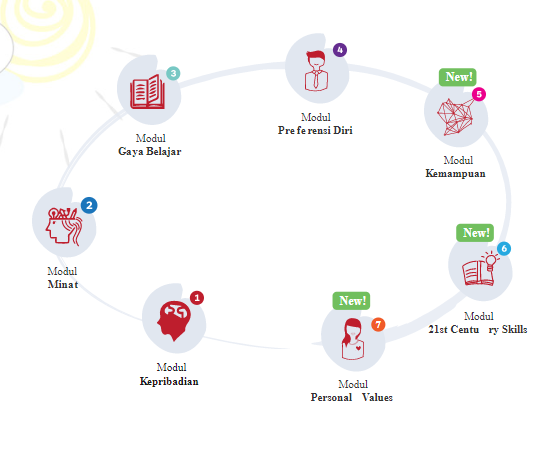
\includegraphics[width = 12cm, height = 12cm]{Gambar/gambar31.PNG}
    \caption{7 Dimensi Profil Siswa}
    \label{gambar31}
\end{figure}

Pada sistem ini, telah dilakukan beberapa analisis dan hasilnya sebagai berikut :

\begin{enumerate}
    \item \textit{Website} \url{https://rencanamu.id} adalah sebuah \textit{platform} persiapan kuliah dan karier \textit{online} berbasis data didukung oleh teknologi \textit{People Science} untuk membantu siswa dalam merancang dan mempersiapkan masa depan mereka. 
    
    \item Perlu melakukan registrasi atau \textit{login} kedalam sistem.
    
    \item Gambar \ref{gambar32} merupakan tampilan awal setelah registrasi atau \textit{login}.
    
    \begin{figure}[H]
        \centering
        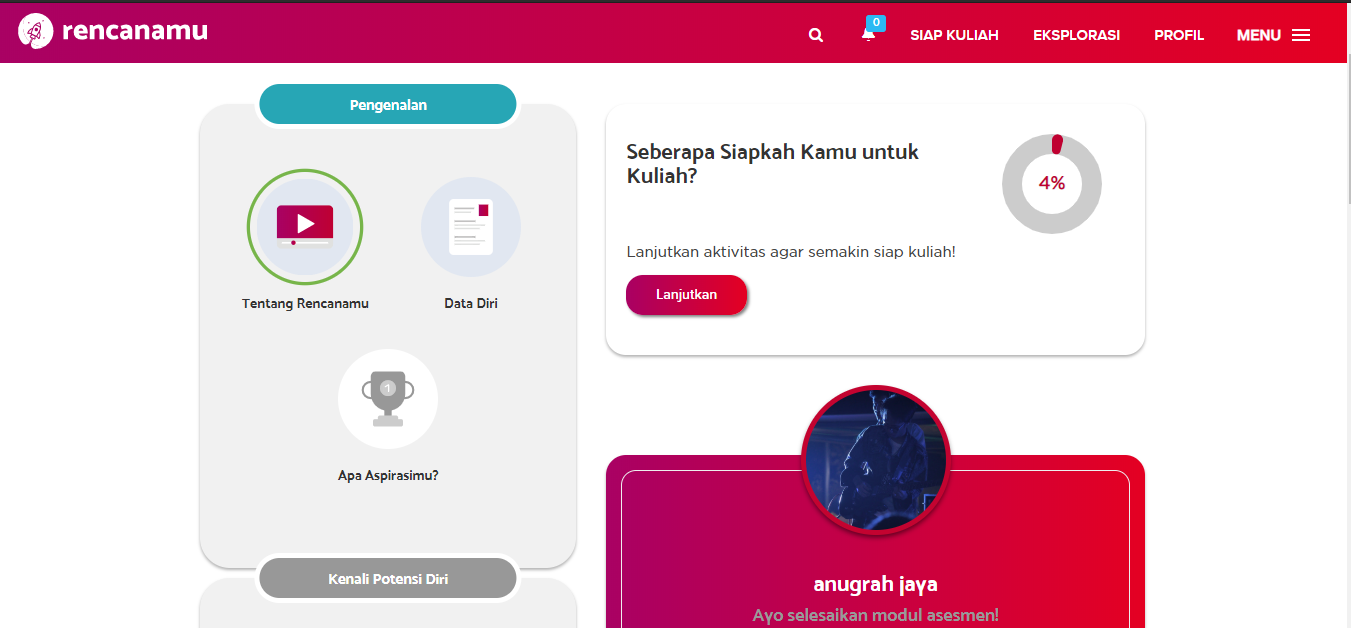
\includegraphics[width = 10cm, height = 6 cm]{Gambar/gambar32.PNG}
        \caption{Tampilan setelah registrasi atau \textit{login}}
        \label{gambar32}
    \end{figure}
    
    \item Gambar \ref{gambar33}, Gambar \ref{gambar34}, dan Gambar \ref{gambar35} adalah beberapa modul yang harus dikerjakan.
    
    \begin{figure}[H]
        \centering
        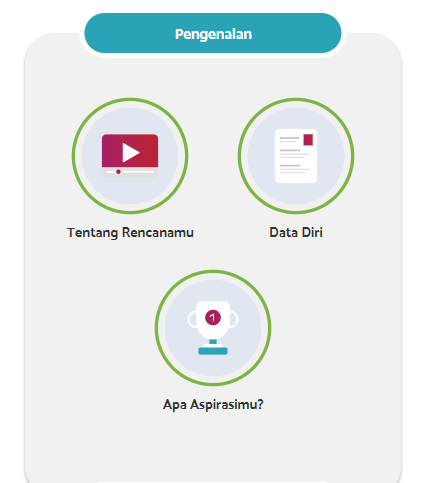
\includegraphics[width = 7cm, height = 10cm ]{Gambar/gambar33.PNG}
        \caption{Modul Pengenalan}
        \label{gambar33}
    \end{figure}
    
    \begin{figure}[H]
        \centering
        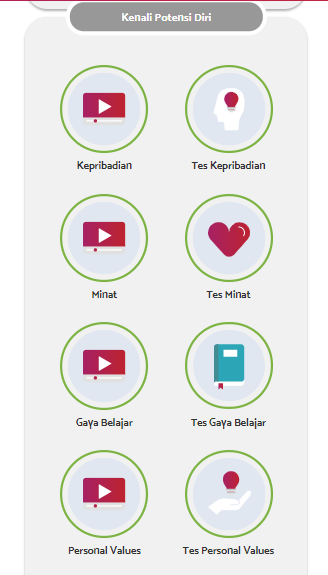
\includegraphics[width = 7cm, height = 11cm ]{Gambar/gambar34.PNG}
        \caption{Modul Potensi Diri}
        \label{gambar34}
    \end{figure}
    
    \begin{figure}[H]
        \centering
        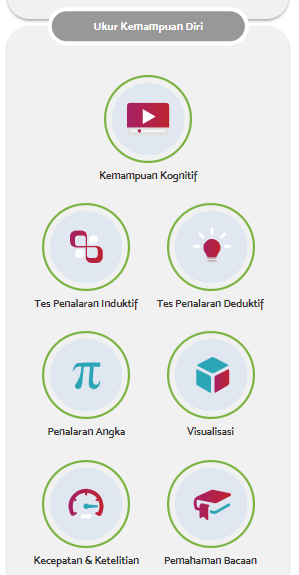
\includegraphics[width = 7cm, height = 11cm ]{Gambar/gambar35.PNG}
        \caption{Modul Ukur Kemampuan Diri}
        \label{gambar35}
    \end{figure}
    
    \item Gambar \ref{gambar36} adalah contoh hasil rekomendasikan yang diberikan sistem berdasarkan modul yang sudah dikerjakan.
    
    \begin{figure}[H]
        \centering
        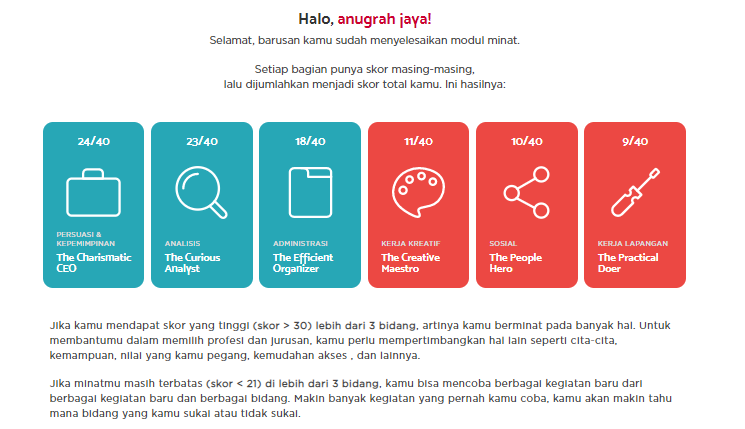
\includegraphics[width = 7cm, height = 10cm ]{Gambar/gambar36.PNG}
        \caption{Hasil Rekomendasi}
        \label{gambar36}
    \end{figure}
    
\end{enumerate}

\textit{Website} \url{https://rencanamu.id} memiliki kesamaan dengan sistem yang dibangun yaitu memberikan rekomendasi program studi untuk anak SMA. Perbedaannya pada \textit{website} \url{https://rencanamu.id} tidak menampilkan prediksi IPK dan harus mengisi beberapa modul untuk mendapatkan rekomendasi program studi. 

\section{\textit{Preprocessing} Data Mahasiswa}
\label{sec:preprocessing}
Data mahasiswa yang digunakan adalah data mahasiswa Universitas Katolik Parahyangan dengan jalur penerimaan Penelurusan dan Kemampuan atau PMDK pada tahun 2013-2018. Pada data yang digunakan terdapat beberapa atribut yang tidak dapat digunakan seperti No.PMB,  kota asal sekolah, dan provinsi asal sekolah. Atribut yang tidak dapat digunakan akan dihapus dan data akan dipisahkan menjadi dua \textit{file} mahasiswa dan nilai untuk setiap program studi yang ada. \textit{prepocessing} dilakukkan menggunakan Python. Berikut langkah-langkah dalam \textit{preprocessing} :

\begin{enumerate}
    \item Membaca file .csv yang berisikan data mahasiswa pada fakultas tertentu.
    
    \item Membuat dataframe untuk menampung data mahasiswa dan nilai.
    
    \item Menginisialisasikan batas \textit{looping}, id\_user, id\_nilai, dan asal jurusan.
    
    \item Menambahkan data mahasiswa berupa NPM, id\_prodi, asal jurusan, dan IPK pada dataframe mahasiswa.
    
    \item Mengubah \textit{range} nilai menjadi GPA (\textit{Grade Point Average}) dan menghitung nilai rata-rata untuk setiap nilai mata pelajaran.
    
    \item Menambahkan data GPA, rata-rata nilai, dan id\_user pada dataframe nilai.
    
    \item Menyimpan dataframe mahasiswa dan nilai menjadi .csv.
\end{enumerate}

Hasil \textit{file} .csv nantinya akan di\textit{import} pada basis data yang akan digunakan pada sistem.  

\section{Pemilihan Algoritma Sistem Rekomendasi}
Berdasarkan teori \ref{teknik rekomendasi} yang menjelaskan mengenai teknik-teknik yang dapat digunakan untuk membangun sistem rekomendasi, teknik \textit{collaborative filtering} adalah teknik yang dapat digunakan untuk memberikan rekomendasi berupa program studi kepada calon mahasiswa berdasarkan kesamaan dengan pengguna lain. Berikut merupakan beberapa hal mengapa memilih teknik \textit{collaborative filtering} :

\begin{enumerate}
    \item \textit{Collaborative filtering} menghasilkan rekomendasi item yang spesifik untuk pengguna berdasarkan peringkat tanpa memerlukan informasi tambahan mengenai item ataupun pengguna.
    
\end{enumerate}

Teknik \textit{collaborative filtering} memiliki beberapa kekurangan diantaranya : 

\begin{enumerate}
    \item Rekomendasi yang diberikan mengambil data yang cukup banyak dari basis data sehingga membutuhkan memori yang besar.
    
    \item Tidak bisa memberikan rekomendasi untuk item yang tidak pernah diberikan \textit{rating} oleh pengguna.
    
    \item Pengguna harus memberikan \textit{rating} untuk beberapa atribut agar bisa diberikan rekomendasi.
    
\end{enumerate}

Pada sistem yang dibangun, akan memberikan rekomendasi berdasarkan nilai raport beberapa mata pelajaran siswa pada kelas 10 dan 11 yang digunakan untuk PMDK. Mata pelajaran yang digunakan adalah Matematika, Bahasa Indonesia, Bahasa Inggris, Fisika, Kimia, dan Pendidikan Kewarganegaraan. Rekomendasi program studi berdasarkan asal jurusan saat SMA, misalnya siswa IPA akan diberikan rekomendasi program studi IPA.


\section{Contoh Perhitungan Pearson Correlation}
Berdasarkan \ref{user-based} terdapat langkah-langkah perhitungan dari \textit{user-based}. Tabel \ref{tab:data mahasswa} merupakan contoh data mahasiswa.

\begin{table}[H]
    \centering
    \renewcommand{\arraystretch}{1.5}
    \begin{tabular}{|l|c|c|c|c|c|}
        \hline
        MP\slash Semester & 101 & 102 & 111 & 112 & AVG \\
        \hline 
        Matematika & 2.6 & 2.9 & 2.95 & 2.75 & 2.8 \\
        \hline 
        Bahasa Indonesia & 0 & 0 & 0 & 0 & 0 \\
        \hline 
        Bahasa Inggris & 2.95 & 3 & 2.85 & 2.95 & 2.9375 \\
        \hline 
        PKN & 0 & 0 & 0 & 0 & 0 \\
        \hline
    \end{tabular}
    \caption{Contoh data mahasiswa dalam bentuk GPA}
	\label{tab:data mahasswa}
\end{table}

Berikut merupkan contoh langkah-langkah perhitungan :

\begin{enumerate}
    \item Menghitung nilai rata-rata \textit{rating}.
    
    \begin{table}[H]
    \centering
    \renewcommand{\arraystretch}{1.5}
    \begin{tabular}{|l|c|c|c|c|c|c|}
        \hline
        MP\slash Semester & 101 & 102 & 111 & 112 & Rumus & AVG \\
        \hline 
        Matematika & 2.9 & 3.4 & 3.4 & 2.9 & $\frac{2.9 + 3.4 +3.4 + 2.9}{4}$ & 3.15 \\
        \hline 
        Bahasa Indonesia & 2.95 & 2.9 & 3.9 & 3.4 & $\frac{2.95 + 2.9 + 3.9 + 3.4}{4}$ & 3.2875 \\
        \hline 
        Bahasa Inggris & 3.3 & 3.35 & 3.25 & 2.9 & $\frac{3.3 + 3.35 + 3.25 + 2.9}{4}$ & 3.2 \\
        \hline 
        PKN & 3.4 & 2.9 & 3.35 & 2.35 & $\frac{3.4 + 2.9 + 3.35 + 2.35}{4}$ & 3 \\
        \hline
    \end{tabular}
    \caption{Contoh data siswa dalam bentuk GPA}
	\label{tab:data siswa}
\end{table}

    \item Menghitung kesamaan atau similaritas.
    
    \begin{table}[H]
        \centering
        \renewcommand{\arraystretch}{1.5}
        \begin{tabular}{|c|c|c|c|c|}
            \hline
            No & Rumus & Matematika & Rumus & Bahasa Inggris \\
            \hline
            \multirow{2}{*}{1} & $(2.9-3.15)*$ & 0.5    & $(3.3-3.2)*$ & 0.00125\\
            & $(2.6-2.8)$ & & $(2.95-2.9375)$ &  \\
            \hline
            \multirow{2}{*}{2} & $(3.4-3.15)*$ & 0.025  & $(3.35-3.2)*$ & 0.009375 \\
            & $(2.9-2.8)$ & & $(3-2.9375)$ &  \\
            \hline
            \multirow{2}{*}{3} & $(3.4-3.15)*$ & 0.0375 & $(3.25-3.2)*$ & -0.004375 \\
            & $(2.95-2.8)$ &  & $(2.85-2.9375)$ &  \\
            \hline
            \multirow{2}{*}{4} & $(2.9-3.15)*$ & 0.0125 & $(2.9-3.2)*$ & -0.00375 \\
            & $(2.75-2.8)$ &  & $(2.95-2.9375)$ &  \\
            \hline
            \multirow{2}{*}{Sigma} & $0.5 + 0.025 +$ & 0.125 & $0.00125 + 0.009375 +$ & 0.0025 \\
            & $0.0375 + 0.0125$ & & $-0.004375 + -0.00375$ &  \\
            \hline
            \multicolumn{3}{|c|}{Hasil} & $0.125+0.0025$ & 0.1274 \\
            \hline
        \end{tabular}
        \caption{Nilai kovariasi mahasiswa dan siswa}
        \label{tab:kovariasi}
    \end{table}
    
    \begin{table}[H]
        \centering
        \renewcommand{\arraystretch}{1.5}
        \begin{tabular}{|c|c|c|c|c|}
    		\hline
    		No & Rumus & Matematika & Rumus & Bahasa Inggris\\
    		\hline
    		1 & $(2.9-3.15)^2$ & 0.0625 & $(3.3-3.2)^2$ & 0.01 \\
    		\hline
    		2 & $(3.4-3.15)^2$ & 0.0625 & $(3.35-3.2)^2$ & 0.0225 \\
    		\hline
    		3 & $(3.4-3.15)^2$ & 0.0625 & $(3.25-3.2)^2$ & 0.0025 \\
    		\hline
    		4 & $(2.9-3.15)^2$ & 0.0625 & $(2.9-3.2)^2$ & 0.09 \\
    		\hline
    		\multirow{2}{*}{Sigma} & 0.0625+0.0625+ & 0.25 & 0.01+0.0225+ & 0.125\\
    		& 0.0625+0.0625 & & 0.0025+0.09 & \\
    		\hline
    		\multicolumn{3}{|c|}{Hasil} & $\sqrt{0.25+0.125}$ & 0.612372436 \\
    		\hline
        \end{tabular}
        \caption{Standar Deviasi Siswa}
    	\label{tab:sd_siswa}
    \end{table}
    
    \begin{table}[H]
        \centering
        \renewcommand{\arraystretch}{1.5}
        \begin{tabular}{|c|c|c|c|c|}
    		\hline
    		No & Rumus & Matematika & Rumus & Bahasa Inggris\\
    		\hline
    		1 & $(2.6-2.8)^2$ & 0.04 & $(2.95-2.9375)^2$ & 0.00015625 \\
    		\hline
    		2 & $(2.9-2.8)^2$ & 0.01 & $(3-2.9375)^2$ & 0.00390625 \\
    		\hline
    		3 & $(2.95-2.8)^2$ & 0.0225 & $(2.85-2.9375)^2$ & 0.00765625 \\
    		\hline
    		4 & $(2.75-2.8)^2$ & 0.0225 & $(2.95-2.9375)^2$ & 0.00015625
     \\
    		\hline
    		\multirow{2}{*}{Sigma} & 0.04+0.01+ & 0.075 & 0.0.000156250.00390625+ & 0.011875\\
    		& 0.0225+0.0225 & & 0.00765625+0.00015625 & \\
    		\hline
    		\multicolumn{3}{|c|}{Hasil} & $\sqrt{0.075+0.011875}$ & 0.294745653	 \\
    		\hline
        \end{tabular}
        \caption{Standar Deviasi Mahasiswa}
    	\label{tab:sd_mahasiswa}
    \end{table}
    
    \begin{table}[H]
        \centering
        \renewcommand{\arraystretch}{1.5}
        \begin{tabular}{|c|c|c|c|}
            \hline
            No & Rumus & Kesamaan & IPK \\ 
            \hline
            1 & $\frac{0.1275}{0.612372436*0.294745653}$ & 0.706394228 & 3.11\\
            \hline
            2 & $\frac{0.0125}{0.612372436*0.2343242}$ & 0.08711185 & 2.9 \\
            \hline
            3 & $\frac{0.2}{0.612372436*0.543242}$ & 0.601202838 & 3 \\
            \hline
            4 & $\frac{0.125}{0.612372436*0.432343}$ & 0.472134729 & 3.2\\
            \hline
            5 & $\frac{0.05}{0.612372436*0.242345}$ & 0.336914969 & 3.4\\
            \hline
        \end{tabular}
        \caption{Contoh Perhitungan kesamaan}
        \label{tab:kesamaan}
    \end{table}
    
    \item Memilih nilai kesamaan atau similaritas yang bernilai lebih dari 0.
    
    Berdasarkan langkah nomor 2, maka nilai kesamaan pada tabel \ref{tab:kesamaan} semuanya dapat digunakan untuk prediksi.
    
    \item Menghitung nilai prediksi.
    
    \begin{table}[H]
        \centering
        \renewcommand{\arraystretch}{1.5}
        \begin{tabular}{|c|c|c|c|}
            \hline
            No & Kesamaan & Rumus & Kesamaan*IPK \\
            \hline
            1 & 0.706394228 & 0.706394228*3.11 & 2.196886049 \\
            \hline
            2 & 0.08711185 & 0.08711185*2.9 &  0.252624364 \\
            \hline
            3 & 0.601202838 & 0.601202838*3 & 1.803608514 \\
            \hline
            4 & 0.472134729 & 0.472134729*3.2 & 1.510831133 \\
            \hline
            5 & 0.336914969 & 0.336914969*3.4 & 1.145510893 \\
            \hline
            Sigma & 2.203758614 & - & 6.909460954 \\
            \hline
            \multicolumn{2}{|c|}{Hasil} & $\frac{6.909460954}{2.203758614}$ & 3.13530752\\
            \hline
        \end{tabular}
        \caption{Contoh hasil Prediksi}
        \label{tab:prediksi}
    \end{table}
\end{enumerate}

\section{Contoh Perhitungan Metode Evaluasi Sistem Rekomendasi}
\label{sec:contoh perhitungan evaluasi}

Berdasarkan penjelasan mengenai sistem rekomendasi yang dibahas pada bab \ref{chap:teori} bagian \ref{sec:aplikasi dan evaluasi}. Salah satu bagian terpenting adalah evaluasi. Evalusi pada sistem rekomendasi dilakukkan untuk mendapatkan akurasi dari hasil prediksi yang diberikan. Akurasi merupakan salah satu aspek yang sering dijadikan acuan untuk rekomendasi yang digunakan. Dalam melakukan pengujian akurasi bisa menggunkan metode \textit{Mean Absolute Error} (MAE) dan \textit{Root Mean Square Error} (RMSE). Berikut merupakan contoh penerapan kedua metode yang akan disajikan dalam tabel \ref{tab:tabel data mae dan rmse} :

\begin{longtable}[H]{|c|c|c|c|c|c|c|c|}
    %\centering
    %\begin{tabular}{|c|c|c|c|c|c|c|c|}
        \hline
        \multirow{2}{2em}{No} & Item & Pengguna & Penilaian Asli & Prediksi Sistem  & $r_{u,i}-\hat{r}_{u,i}$ & $\mid r_{u,i}-\hat{r}_{u,i} \mid$ & $(r_{u,i}-\hat{r}_{u,i})^2$ \\ 
        & & & $r_{u,i}$ & $\hat{r}_{u,i}$ & & &\\
        \hline
        1 & 110 & 1 & 3.4 & 3.5 & -0.1 & 0.1 & 0.01\\
        \hline
        2 & 120 & 30 & 3.3 & 3.1 & 0.2 & 0.2 & 0.04\\
        \hline
        3 & 130 & 56 & 3 & 2.8 & 0.2 & 0.2 & 0.04\\
        \hline
        4 & 200 & 65 & 2.9 & 3.1 & -0.2 & 0.2 & 0.04\\
        \hline
        5 & 310 & 76 & 3.1 & 2.8 & 0.3 & 0.3 & 0.09\\
        \hline
        6 & 320 & 87 & 3.2 & 3 & 0.2 & 0.2 & 0.04\\
        \hline
        7 & 330 & 99 & 2.8 & 3 & -0.2 & 0.2 & 0.04\\
        \hline
        8 & 410 & 102 & 3.4 & 3.5 & -0.1 & 0.1 & 0.01\\
        \hline
        9 & 420 & 167 & 3.1 & 3.5 & -0.4 & 0.4 & 0.16\\
        \hline
        10 & 510 & 189 & 2.8 & 3.1 & -0.3 & 0.3 & 0.09\\
        \hline
        11 & 610 & 298 & 3.1 & 2.9 & 0.2 & 0.2 & 0.04\\
        \hline
        12 & 620 & 344 & 3.4 & 2.9 & 0.5 & 0.5 & 0.25\\
        \hline
        13 & 630 & 365 & 3.1 & 3 & 0.1 & 0.1 & 0.01\\
        \hline
        14 & 710 & 465 & 2.9 & 3 & -0.1 & 0.1 & 0.01\\
        \hline
        15 & 720 & 477 & 3.4 & 3.5 & -0.1 & 0.1 & 0.01\\
        \hline
        16 & 730 & 480 & 3.4 & 3.6 & -0.2 & 0.2 & 0.04\\
        \hline
        \multicolumn{6}{|c|}{Jumlah} & 3.4 & 0.92 \\
        \hline
    %\end{tabular}
    \caption{Tabel Data MAE dan RMSE}
    \label{tab:tabel data mae dan rmse}
\end{longtable}

Berdasarkan data pada tabel \ref{tab:tabel data mae dan rmse} jika dihitung dengan persamaan MAE yaitu :

\begin{equation}
    MAE = \frac{1}{n} * \Sigma \mid r_{u,i}-\hat{r}_{u,i} \mid
\end{equation}

maka akan didapatkan hasil pengimplementasian dari rumus MAE sebagai berikut :

\begin{equation}
    MAE = \frac{1}{16} * 3.4 = 0.2125 
\end{equation}

Berdasarkan data pada tabel \ref{tab:tabel data mae dan rmse} jika dihitung dengan persamaan RMSE yaitu :

\begin{equation}
    RMSE = \sqrt{\frac{1}{n} * \Sigma (r_{u,i}-\hat{r}_{u,i})^2}
\end{equation}

maka akan didapatkan hasil pengimplementasian dari rumus RMSE sebagai berikut :

\begin{equation}
    RMSE = \sqrt{\frac{1}{16} * 0.91} = 0.0575
\end{equation}

\section{Analisis Kebutuhan Sistem}
\label{analisis kebutuhan sistem}
Pada sistem yang akan dibangun, memiliki kebutuhan-kebutuhan perangkat lunak seperti : \textit{Use Case} dan Rancangan Basis Data.

% perlu atau engga ? kata bu mar ga terlalu perlu
\subsection{Diagram \textit{Use Case}}
Pada sistem yang akan dibangun terdapat satu aktor yaitu Siswa/i. Siswa/i ini adalah calon mahasiswa kelas XI yang merupakan target dari sistem yang akan dibangun. Terdapat 4 langkah yang harus dilakukan, yaitu :

\begin{enumerate}
    \item Pendefinisian Aktor
    
    \begin{table}[H]
        \centering
        \begin{tabular}{|c|p{4cm}|p{8cm}|}
            \hline
            No & Aktor & Deskripsi  \\
            \hline
            1 & Siswa/i &  Siswa/i adalah orang yang akan diberikan rekomendasi program studi yang ada di Universitas Parahyangan.\\
            \hline
        \end{tabular}
        \caption{Pendefinisian Aktor}
        \label{tab:pendefsian aktor}
    \end{table}
    
    \item Pendefinisian \textit{Use Case}
    
    \begin{longtable}[H]{|c|p{4cm}|p{8cm}|}
        %\centering
        %\begin{tabular}
            \hline
            No & \textit{Use Case} & Deskripsi  \\
            1 & Memilih Jurusan SMA & Merupakan proses untuk memilih jurusan saat SMA. \\
            \hline
            2 & Mengisi Nilai Rapor & Merupakan proses untuk mengisi nilai beberapa nilai mata pelajaran sesuai dengan jurusan saat SMA. \\ 
            \hline
        %\end{tabular}
        \caption{Pendefinisian \textit{Use Case}}
        \label{tab:pendefinisian use case}
    \end{longtable}
    
    \item Pembuatan \textit{Use Case} Skenario
    
    \begin{longtable}[H]{|p{6.5cm}|p{6.5cm}|}
        %\centering
        %\begin{tabular}
            \hline
            Aksi Aktor & Reaksi Sistem \\
            \hline
            \multicolumn{2}{|c|}{Skenario Normal}\\
            \hline
            1. Memilih jurusan saat SMA. & \\
            \hline
             & 2. Mengarahkan kepada form sesuai jurusan SMA. \\
            \hline
        %\end{tabular}
        \caption{Skenario Memilih Jurusan SMA}
        \label{tab:skenario memilih jurusan sma}
    \end{longtable}
    
    \begin{longtable}[H]{|p{6.5cm}|p{6.5cm}|}
        %\centering
        %\begin{tabular}
            \hline
            \multicolumn{2}{|c|}{Skenario Normal}\\
            \hline
            1. Mengisi nilai sesuai nilai rapor. & \\
            \hline
            & 2. Memeriksa valid tidaknya data yang dimasukkan. \\
            \hline
            & 3. Memeriksa range nilai.\\
            \hline
            4. Klik tombol submit. & \\
            \hline
            & 5. Mengarahkan kepada halaman hasil rekomendasi.\\
            \hline
            \multicolumn{2}{|c|}{Skenario Alternatif}\\
            \hline
             1. Mengisi nilai yang tidak valid. & \\
            \hline
            & 2. Memeriksa valid tidaknya data yang dimasukkan. \\
            \hline
            & 3. Memberikan pesan data tidak valid.\\
            \hline
            4. Mengisi nilai sesuai nilai rapor yang valid. & \\
            \hline
            & 5. Memeriksa \textit{range} nilai.\\
            \hline
            & 6. Memberikan pesan \textit{range} tidak sesuai.\\
            \hline
            7. Mengisi nilai sesuai \textit{range}. &\\
            \hline
            & 8. Memeriksa \textit{range} nilai.\\
            \hline
            9. Klik tombol submit. & \\
            \hline
            & 10. Mengarahkan kepada \textit{page} hasil rekomendasi.\\
            \hline
        %\end{tabular}
        \caption{Skenario Mengisi Nilai Rapor}
        \label{tab:skenario mengisi nilai rapor}
    \end{longtable}
    
    \item Menggambarkan Diagram \textit{Use Case}
    
    \begin{figure}[H]
        \centering
        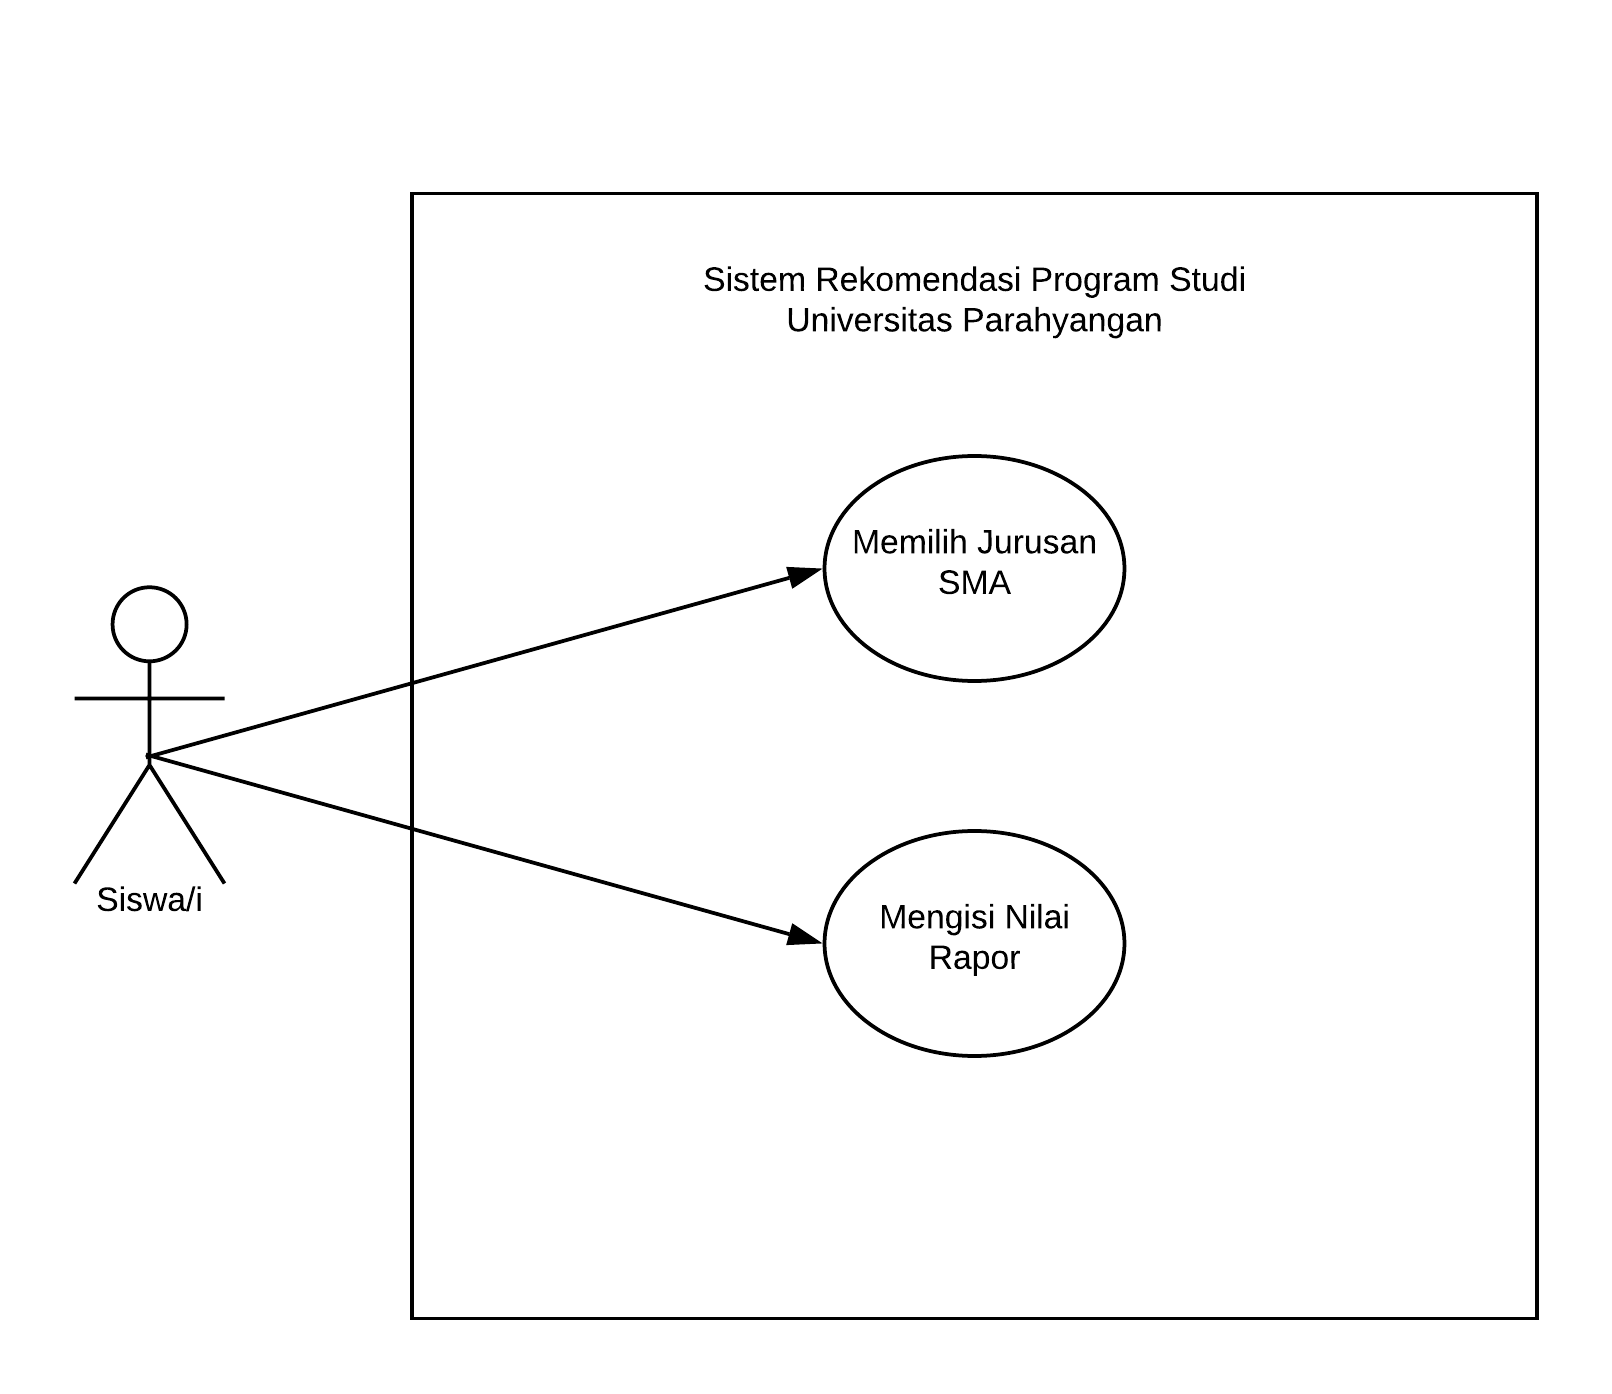
\includegraphics[width = 14cm, height = 14cm]{Gambar/gambar38.png}
        \caption{Diagram \textit{Use Case} Sistem Rekomendasi}
        \label{fig:diagram use case}
    \end{figure}
\end{enumerate}

\subsection{Rancangan Basis Data}
\label{rancangan basis data}
% erd, table, skema relasi

\subsubsection{Diagram ERD}
\label{diagram erd}

\begin{figure}[H]
    \centering
    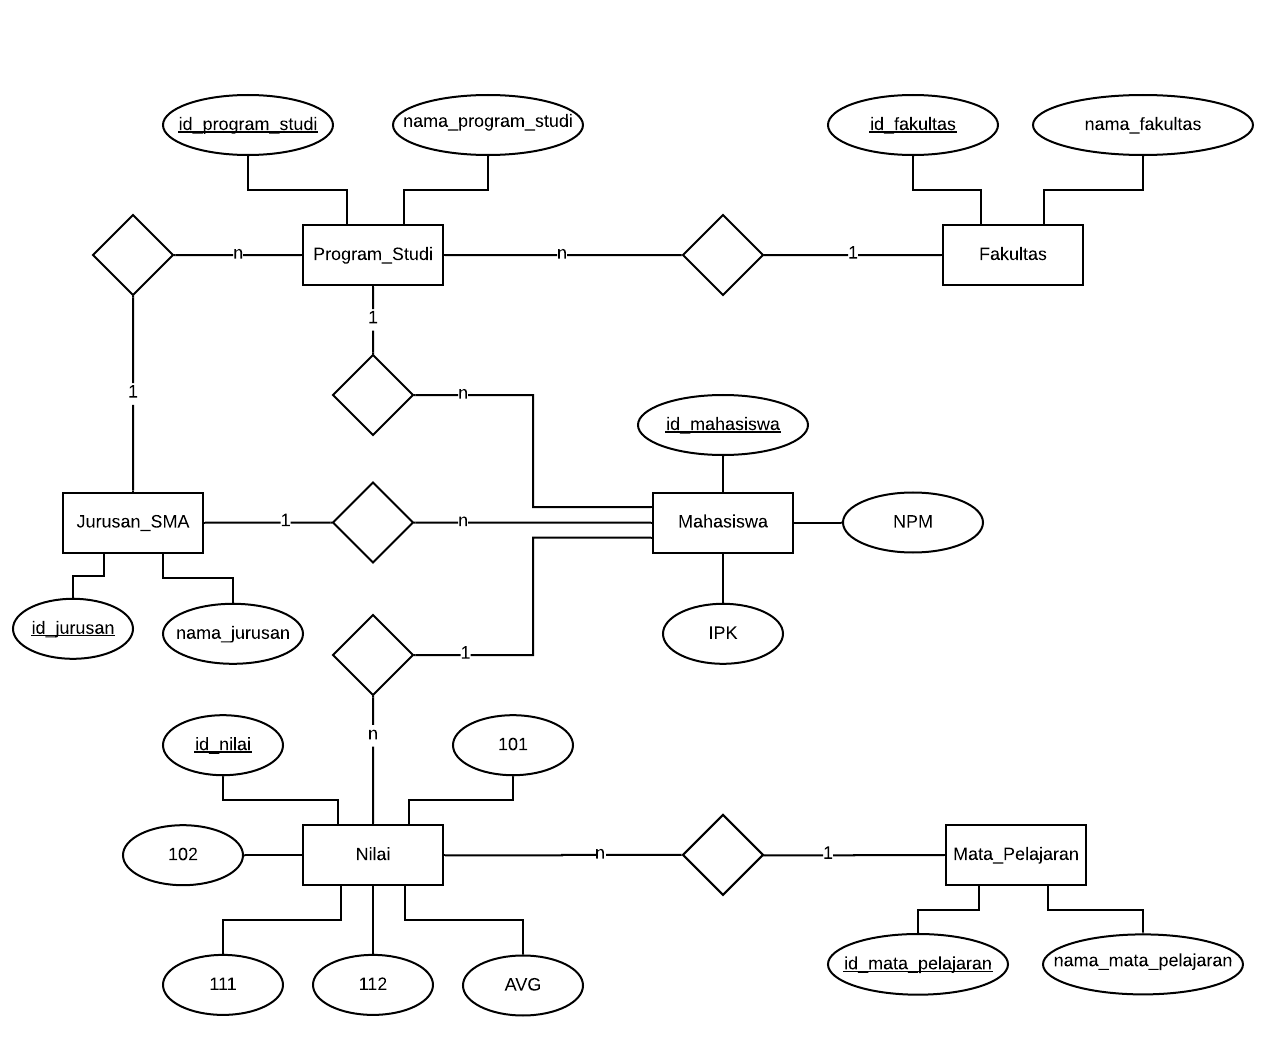
\includegraphics[width = 16cm, height = 14cm ]{Gambar/gambar37.png}
    \caption{Diagram ERD Sistem Rekomendasi}
    \label{fig:diagram erd}
\end{figure}

Berikut merupakan entitas dan atribut gambar \ref{fig:diagram erd} yang akan digunakan pada sistem yang akan dibangun :

\begin{enumerate}
    \item Jurusan\_SMA memiliki atribut id\_jurusan dan nama jurusan.
    
    \item Fakultas memiliki atribut id\_fakultas dan nama\_fakultas.
    
    \item Program\_Studi memiliki atribut id\_program\_studi dan nama\_program\_studi.
    
    \item Mahasiswa memiliki atribut id\_mahasiswa, NPM, dan IPK.
    
    \item Mata\_Pelajaran memiliki atribut id\_mata\_pelajaran dan nama\_mata\_pelajaran.
    
    \item Nilai memiliki atribut id\_nilai, 101, 102, 111, 112, dan AVG. 
\end{enumerate}



